\section{Running \CNAME\label{sec:running}\index{Running \CNAME}}

\CNAME\ is run from the console window (i.e., the command line) on \I{Microsoft Windows} or from a terminal window on \I{Linux}. \CNAME\ uses information from input data files -- the \emph{\config\index{Input configuration file}} being the key file. 

The \config\ is compulsory and defines the model structure, processes, observations, parameters (both the fixed parameters and the parameters to be estimated)\index{Estimable parameters}, and the reports (outputs) requested. The following sections  describe how to construct the \CNAME\ configuration file. By convention, the name of the \config\ ends with the suffix \texttt{.csl2}. However, any file name is acceptable. Note that the \config\ can `include' other files as a part of its syntax. Collectively, these are called the \config.

Other input files can, in some circumstances, be supplied depending on what is required. For example, an input file can define the starting point for estimation, or points from which to simulate observations, or points from which to run projections.

Simple command line arguments\index{Command line arguments} are used to determine the actions or \emph{tasks}\index{Tasks} of \CNAME, e.g. to run a model with a set of parameter values, estimate parameter values (either point estimates or MCMC), project quantities into the future or simulate observations. Hence, the \emph{command line arguments} define the \emph{task}. For example, \texttt{-r} is the \emph{run}, \texttt{-e} is the \emph{estimation}, and \texttt{-m} is the \emph{MCMC} task. The \emph{command line arguments} are described in Section \ref{sec:command-line-arguments}.

\subsection{\I{Using \CNAME}}

To use \CNAME, open a console (i.e. the command prompt) window (Microsoft Windows) or a terminal window (Linux). Navigate to a directory of your choice, where your \config s are located. Then enter \cname\ with any arguments (see Section \ref{sec:command-line-arguments} for the the list of possible arguments) to start your \CNAME\ job running. \CNAME\ will print output to the screen and return you to the command prompt when the job has completed. Note that the \CNAME\ executable (binary) and shared libraries (extension \texttt{.dll}) must be either in the same directory as the \config s or in your systems \texttt{PATH}. The \CNAME\ installer should update your path on Windows in any case, but see your operating system documentation for help identifying or modifying your \texttt{PATH}.


\subsection{The \config\label{sec:config-files}}\index{Input configuration file}

The \config\ is made up of four broad sections; the description of the population structure and parameters (the population section), the estimation methods and variables (the estimation section), the observations and their associated likelihoods (the observation section), and the outputs and reports that \CNAME\ will return (the report section). The \config\ is made up of a number of commands (many with subcommands) which specify various options for each of these components.

The command and subcommand definitions in the \config\ can be extensive (especially when you have a model that has many observations), and can result in a \config\ that is long and difficult to navigate. To aid readability and flexibility, we can use the \config\ command !\texttt{\emph{include}} \texttt{\emph{file}}  (e.g. Figure~\ref{fig:config_file_1}). The command causes an external file, \argument{\emph{file}}, to be read and processed, exactly as if its contents had been inserted in the main \config\ at that point\index{Including external files}. The file name must be a complete file name with extension, but can use either a relative or absolute path as part of its name. Note that included files can also contain !\texttt{\emph{include}} commands. See Section \ref{sec:general-syntax} for more detail.


\vspace*{3mm}
\begin{figure}[htp]
	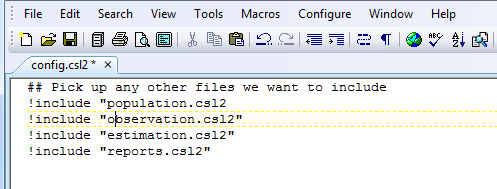
\includegraphics[scale=1]{Figures/config.png}
	\caption{\textbf{Example of using the \config\ command !\texttt{\emph{include}}
	 \texttt{\emph{file}} .}}\label{fig:config_file_1}
\end{figure}
%\vspace*{1mm}

\subsection{\I{Redirecting standard output}\label{sec:redirecting-stdout}}

\CNAME\ uses the \texttt{standard output}\index{standard output} stream to display run-time information. The \I{standard error} stream is used by \CNAME\ to output the program exit status and run-time errors. We suggest redirecting both the standard output and standard error into files\index{Redirecting standard out}\index{Redirecting standard error}. With the bash shell (on Linux systems), you can do this using the command structure,

\begin{verbatim} (casal2 [arguments] > out) >& err &\end{verbatim}

It may be useful to redirect the standard input, especially if you're using \CNAME\ inside a batch job software, i.e. 

\begin{verbatim} (casal2 [arguments] > out < /dev/null) >& err &\end{verbatim}

On Microsoft Windows systems, you can redirect to standard output using,

\begin{verbatim} casal2 [arguments] > out\end{verbatim}

And, on some Microsoft Windows systems (e.g., Windows10), you can redirect to both standard output and standard error, using the syntax, 

\begin{verbatim} casal2 [arguments] > out 2> err\end{verbatim}

Note that \CNAME\ outputs a few lines of header information to the output (e.g. Figure~\ref{fig:log_file_1}). The header\index{Output header information} consists of the program name and version, the arguments passed to \CNAME\ from the command line, the date and time that the program was called (derived from the system time), the user name, and the machine name (including the operating system and the process identification number). These can be used to track outputs as well as identifying the version of \CNAME\ used to run the model.

\begin{figure}[htp]
	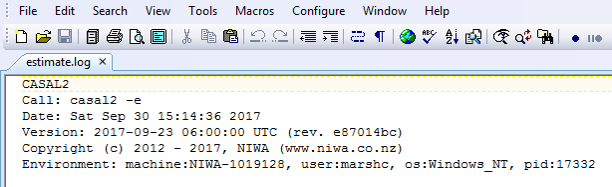
\includegraphics[scale=1]{Figures/eglog.png}
	\caption{\textbf{Example of output file header information.}}\label{fig:log_file_1}
\end{figure}

\vspace*{4mm}

\subsection{\I{Command line arguments}\label{sec:command-line-arguments}}

The call to \CNAME\ is of the following form: 

\texttt{\cname [-c \emph{config\_file}] [\emph{task}] [\emph{options}]}

where, 

\begin{description}
  \item [\texttt{-c \emph{config\_file}}] Define the \config\ for \CNAME\ (if omitted, \CNAME\ looks for a file named \texttt{config.csl2})
\end{description}

and where \emph{task} must be one of the following (\textbf{[]} indicates a secondary label to call the task, e.g. \textbf{\texttt{-h}} will execute the same task as \textbf{\texttt{--help}}),

\begin{description}
\item [\texttt{-h [--help]}] Display help (this page)
\item [\texttt{-l [--licence]}] Display the reference for the software license (GPL v2)
\item [\texttt{-v [--version]}] Display the \CNAME\ version number

\item [\texttt{-r [--run]}] \emph{Run} the model once using the parameter values in the \config, or optionally, with the values from the file denoted with the command line argument \texttt{-i \emph{file}}

\item [\texttt{-e [--estimate]}] Do a point \emph{estimate} using the values in the \config\ as the starting point for the parameters to be estimated, or optionally, with the start values from an input file specified by the options argument \texttt{-i \emph{file}}

\item [\texttt{-p [--profiling]}] Do a likelihood \emph{profile} using the parameter values in the \config\ as the starting point, or optionally, with the start values from an input file specified by the options argument \texttt{-i \emph{file}}

\item [\texttt{-m [--mcmc]}] Do an \emph{MCMC} estimate using the values in the \config\ as the starting point for the parameters to be estimated, or optionally, with the start values from an input file specified by the options argument \texttt{-i \emph{file}}

\item [\texttt{-f [--projection]}] Project the model \emph{forward} in time using the parameter values in the \config\ as the starting point for the estimation, or optionally,  with the start values from an input file specified by the options argument \texttt{-i \emph{file}} 

\item [\texttt{-s [--simulation]} \emph{number}] \emph{Simulate} the \emph{number} of observation sets using values in the \config\ as the parameter values, or optionally, with the parameter values from an input file specified by the options argument \texttt{-i \emph{file}}
\end{description}

and where the following optional arguments\index{Optional command line arguments} [\emph{options}] may be specified,

\begin{description}
\item [\texttt{-i [--input] \emph{file}}] \emph{Input} one or more sets of free (estimated) parameter values from \texttt{\emph{file}} (see Section \ref{sec:report-syntax} for details about the format of \texttt{\emph{file}})

\item [\texttt{-o [--output]\emph{file}}] \emph{Output} a report of the free (estimated) parameter values in a format suitable for \texttt{-i \emph{file}} (see Section \ref{sec:report-syntax} for details about the format of \texttt{\emph{file}})

\item [\texttt{-g [--seed]\emph{seed}}]  \emph{Seed} the random number \emph{generator} with \texttt{\emph{seed}}, a positive (long) integer value (note, if \texttt{-g} is not specified, then \CNAME\ will  generate a random number seed based on the computer clock time)

\item [\texttt{--loglevel}] arg = \{trace, finest, fine, medium\} (see Section \ref{sec:report-section})

\item [\texttt{--tabular}] Run with \texttt{-r} or \texttt{-f}  command it will print \command{report} in tabular format (see Section \ref{sec:report-section})

\item [\texttt{--single-step}] Run with \texttt{-r}, this additional option will pause the model and ask the user to specify parameters and their values to use for the next iteration (see Section \ref{sec:singlestepping})

\item [\texttt{-q [--query]\emph{object type}}] \emph{Query} an object type to print an extract of the object description and parameter definitions.  An object can be defined as \texttt{\emph{block.type}}, e.g. \texttt{casal2 --query process.recruitment\_constant} will query the constant recruitment block.

\end{description}

\subsection{Constructing the \CNAME\ \config s \label{constructing-config}}\index{Input configuration file syntax}

The model definition, parameters, observations, and reports are specified in \config s:
 
\begin{description}

\item Population input (Section \ref{sec:population-section}) specifies the model structure, population dynamics, and other associated parameters;
\item Estimation input (Section \ref{sec:estimation-section}) defines the objective function, parameters of the model, and the method of estimation (point estimates, Bayesian posteriors, profiles, etc.);
\item Observation input (Section \ref{sec:observation-section}) contains all the observations data available to the model and  describes how the observed values should be formatted, how \CNAME\ calculates the expected values, and the likelihoods available for each type of observation; and
\item Report input (Section \ref{sec:report-section}) specifies any output required.
\end{description}

The command and subcommand syntax to be used in each of these configuration files are listed in Sections \ref{sec:population-syntax} (Population), \ref{sec:estimation-syntax} (Estimation), \ref{sec:observation-syntax} (Observation) and \ref{sec:report-syntax} (Report).

\subsubsection{Commands}\index{Commands}

\CNAME\ has a range of commands that define the model structure, processes, observations, and how tasks are carried out. There are three types of commands, 

\begin{enumerate}
\item Commands that have an argument and do not have subcommands (for example, !\texttt{\emph{include}}\ \argument{\emph{file}})
\item Commands that have a label and subcommands (for example \command{process} must have a label, and has subcommands)
\item Commands that do not have either a label or argument, but have subcommands (for example \command{model})
\end{enumerate}

Commands that have a label must have a unique label, i.e., the label cannot be used on more than one command of that type. The labels can contain alpha numeric characters, period (`.'), underscore (`\_') and dash (`-'). Labels must not contain white-space, or other characters that are not letters, numbers, dash, period or an underscore. For example,

{\small{\begin{verbatim}
@process NaturalMortality
or
!include MyModelSpecification.csl2
		\end{verbatim}}}

\subsubsection{Subcommands}\index{Commands ! Subcommands}

\CNAME\ subcommands are used for defining options and parameter values related to a particular command. Subcommands always take an argument which is one of a specific \emph{type}. The argument \emph{types} acceptable for each subcommand are defined in Section \ref{sec:syntax}, and are summarised below. 

Like commands (\command{command}), subcommands and their arguments are not order specific --- except that that all subcommands of a given command must appear before the next \command{command} block. \CNAME\ may report an error if they are not supplied in this way. However, in some circumstances a different order may result in a valid, but unintended set of actions, leading to possible errors in your expected results.  

The argument type for a subcommand can be either\index{Subcommand argument type}:

\begin{tabular}{ll}
\textbf{switch} & true/false\\ 
\textbf{integer}& an integer number,\\
\textbf{integer vector} & a vector of integer numbers,\\
\textbf{integer range} & a range of integer numbers separated by a colon, e.g. 1994:1996 is \\ & expanded to an integer vector of values (1994 1995 1996),\\
\textbf{constant} & a real number (i.e. double),\\
\textbf{constant vector} & a vector of real numbers (i.e. vector of doubles),\\
\textbf{estimable} & a real number that can be estimated (i.e. estimable double),\\
\textbf{estimable vector} & a vector of real numbers that can be estimated (i.e. vector of estimable \\ & doubles),\\
\textbf{addressable} & a real number that can be referenced but not estimated (i.e. addressable double),\\
\textbf{addressable vector} & a vector of real numbers that can be referenced but not estimated (i.e. vector of addressable \\ & doubles),\\
\textbf{string} & a categorical (string) value, or\\
\textbf{string vector} & a vector of categorical values.
\end{tabular}

Switches are parameters which are either true or false. Enter \emph{true} as \argument{true} or \argument{t}, and \emph{false} as \argument{false} or \argument{f}. 

Integers must be entered as integers (i.e., if \subcommand{year}\ is an integer then use 2008, not 2008.0)

Arguments of type integer vector, integer range, constant vector, estimable vector, addressable vector, or categorical vector must contain one or more entries on a row, separated by white space (tabs or spaces). 

Parameters are defined in the population section and can be specified as estimable with the subcommand type \texttt{estimable} or \texttt{estimable vector}.  These parameters will be estimated if specified as such in the estimation section. If the estimable parameter is not specified in the estimation section it will instead be treated as a contstant (or constant vector). In other words, only estimable parameters can be estimated and \CNAME\ must be explicitly commanded to do so for any particular model run. 

Note that parameters defined as addressable with the subcommand type \texttt{addressable} or \texttt{addressable vector} are usually derived quantities and are not directly estimable. As such, they can be acted upon by the model (e.g. called by various processes; have priors and/or penalties assigned to them), but they do not directly contribute to any estimation within the model

\subsubsection{The command-block format}\index{Command block format}
Each command-block consists of a single command (starting with the symbol \command{}) and, for most commands, a unique label or an argument. Each command is then followed by its subcommands and their arguments, e.g., 

\begin{multicols}{3}
	\begin{description}
		\item \command{command}, or
		\item \subcommand{subcommand} \subcommand{argument}
		\item \subcommand{subcommand} \subcommand{argument}
		\item .
		\item .
		\item etc.
		\item \command{command} \subcommand{argument}, or
		\item \subcommand{subcommand} \subcommand{argument}
		\item \subcommand{subcommand} \subcommand{argument}
		\item .
		\item .
		\item etc.
		\item \command{command} \subcommand{\emph{label}}
		\item \subcommand{subcommand} \subcommand{argument}
		\item \subcommand{subcommand} \subcommand{argument}
		\item .
		\item .
		\item etc.
		\end{description}
	\end{multicols}


Blank lines are ignored, as is extra white space (i.e., tabs and spaces) between arguments. However, to start command block the \command{} character must be the first character on the line and must not be preceded by any white space. Each input file must end with a carriage return.

There is no need to mark the end of a command block. This is automatically recognized by either the end of the file, section, or the start of the next command block (which is marked by the \command{} on the first character of a line). Note, however, that the !\texttt{\emph{include}} is the only exception to this rule (see Section \ref{sec:general-syntax}\index{Command ! Include files} for details of the use of !\texttt{\emph{include}}). 

Commands, sub-commands and arguments in the \config s are not case sensitive. Labels and variable values are case sensitive. Also, on a Linux system, external calls to files are case sensitive (i.e., when using !\texttt{\emph{include}} \subcommand{\emph{file}}, the argument \subcommand{\emph{file}} will be case sensitive). 


\subsubsection{\I{Commenting out lines}}\index{Comments}
Text on a line that follows an \commentline\ is considered to be a comment and is ignored. To comment out a group of commands or subcommands, use a \commentline\ at the beginning of each line to be ignored.

Alternatively, to comment out an entire block or section place a \commentstart\ as the first character on the line to start the comment block, then end it with \commentend. All lines (including line breaks) between \commentstart\ and \commentend\ inclusive are ignored. 
{\small{\begin{verbatim}
		# This is a comment and will be ignored
		@process NaturalMortality
		m 0.2
		/* 
		This block of code 
		is a comment and
		will be ignored
		*/
		\end{verbatim}}}

\subsubsection{Determining \CNAME\ object names\label{sec:object-names}\index{Determining parameter names}\index{Parameter names}}

When \CNAME\ processes an \config\ it translates each command block and each subcommand block into a unique \CNAME\ object, each with a unique object name. For commands, this object name is simply the command label. For subcommands, the object name format is either: 

\begin{description}
\item \texttt{command[label].subcommand} if the command has a label, or
\item \texttt{command.subcommand} if the command has no label, or
\item \texttt{command[label].subcommand\{i\}} if the command has a label and the subcommand arguments are a vector, and we are accessing the  \emph{i}th element of that vector. 
\item \texttt{command[label].subcommand\{i:j\}} if the command has a label, and the subcommand arguments are a vector, and we are accessing the elements from $i$ to $j$ (inclusive) of that vector.
\end{description} 

The unique object name is used to reference that unique object when, for example, estimating, applying a penalty, projecting, time varying or applying a profile. For example, the object name of the Natural mortality rates subcommand \subcommand{m} of the command \command{process} with the label \argument{NaturalMortality} is category related and so, the syntax to reference all m related categories is, 

\texttt{process[NaturalMortality].m}

Or, the syntax to specify a single category for which to apply the natural mortality process is,

\texttt{process[NaturalMortality].m\{female\}}

All labels (object names) are user specified. As such, naming conventions are non-restrictive and can be model specific.


\subsection{\I{Single-stepping \CNAME}\label{sec:singlestepping}}\index{Single\_stepping}\index{single\_stepping section}

Single-stepping means \CNAME\ can `pause' after each year in the annual cycle during a model run, write reports, then wait and process user input of updated estimable parameters for the next year. 

This enables \CNAME\ to implement models that require feedback management simulations or scenarios and can be used, for example, in operational management procedures (OMPs). The single-stepping process can be automated using \R, where \CNAME\ may be controlled by \R\ to update input harvest values (e.g. catches in a fisheries model) to evaluate a particular harvest control rule. 

\subsection{\CNAME\ exit status values\index{Exit status value}}
Whether \CNAME\ completes its task successfully or errors out gracefully, it returns a single exit status value 'completed' to the standard output. Error messages will be printed to the console. When configuration errors are found \CNAME\ will print error messages, along with the associated files and line numbers where the errors were identified, for example,

{\small{\begin{verbatim}
	#1: At line 15 in Reports.csl2: Parameter '{' is not supported
\end{verbatim}}}	